\chapter{DLC}
Jako DLC označujeme tvrdé amorfní uhlíkové (a-C) nebo uhlovodíkové vrstvy (a-C:H), které mají vysoký obsah sp$^3$ vázaného uhlíku. Rozdělení amorfních uhlovodíkových vrstev podle množství vodíku, sp$^2$ a~sp$^3$ uhlíku shrnuje ternární diagram na obrázku \ref{DLCtypes}.

\begin{figure}[btp]
  \centering
  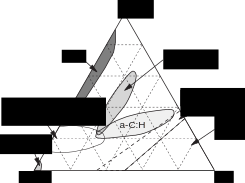
\includegraphics[width=100mm]{grafika/DLCtypes.pdf}
  \caption{Ternární fázový diagram sp$^2$C, sp$^3$C a~H systému \cite{Robertson2002}.}
  \label{DLCtypes}
\end{figure}

Fázový diagram se skládá z několika významných oblastí. Dole vlevo se nachází amorfní grafitový uhlík vyrobený napařováním, případně pyrolýzou uhlovodíkových polymerů, nejedná se nicméně o DLC. Nad ním je s vyšším obsahem sp$^3$ naprašovaný amorfní uhlík a-C, o kterém již můžeme mluvit jako o DLC. Ještě větší obsah sp$^3$ uhlíku má tzv. tetrahedrální amorfní uhlík ta-C. 
Ten je vyráběn iontovými zdroji, které produkují vysoce ionizovaný iontový svazek s úzkým rozdělením energií. Na pravé dolní straně diagramu je naopak oblast, kde je koncentrace vodíku tak velká, že uhlíkové atomy nemohou vytvořit plně propojenou síť a~sloučeniny tak při běžných podmínkách existují pouze v~plynné fázi. 
Hranici této oblasti pak tvoří polymerní uhlovodíkové vrstvy. 

V oblasti uprostřed diagramu se nacházejí amorfní uhlovodíkové vrstvy a-C:H, ty bývají typicky připravovány plazmochemickou depozicí z plynné fáze (PECVD), případně naprašováním grafitu ve vodíkové atmosféře. Poslední oblastí v~grafu jsou husté a~tvrdé a-C:H vrstvy, takzvané amorfní tetrahedrální uhlovodíkové vrstvy (ta-C:H) \cite{Donnet2008a}.    


\section{Růst DLC vrstev}
Důležitým parametrem DLC vrstev je poměr sp$^3$ a~sp$^2$ vázaného uhlíku. Experimentálně se ukázalo, že ideální postup pro dosažení nejvyššího poměru sp$^3$ vazeb je iontové bombardování, přičemž nejvyšší sp$^3$ koncentrace nastávají při depozicích ionty C$^+$ o energiích okolo 140\,eV \cite{Fallon1993}. Následující popis depozičního mechanismu bude prvně proveden pro samotný uhlík (ta-C) a~následně pro a-C:H.

Klíčovým faktem je to, že sp$^2$ vázaný grafit má asi o 50\,\% větší objem než sp$^3$ vázaný diamant. Z toho plyne, že pro větší tlaky dochází k~fázové změně z sp$^2$ na sp$^3$. Zjednodušený základní princip depozice je tedy takový, že díky implantacím vysokoenergetických iontů pod povrch rostoucí vrstvy dochází k~lokálnímu zhuštění materiálu a~k~přechodu z nej\-nižšího energetického stavu sp$^2$ do sp$^3$ \cite{McKenzie1991}.

Podrobnější analýzou se ukazuje, že pro ionty s energiemi cca desítky až stovky elektronvoltů je hloubka implantace  řádově jednotky nanometrů a~ionty ztrácí energii především elastickými srážkami s atomy terče. Srážky můžeme aproximovat jako binární, takže celý proces zastavení iontu lze potom popsat jako řadu po sobě jdoucích nezávislých binárních srážek. Účinný průřez pro srážku závisí na energii iontu a~se stoupající energií klesá. Pro nízké energie proto iont není schopen proniknout povrchem a~skončí na povrchu rostoucí vrstvy v~nejnižším energetickém stavu. Minimální energie, kterou iont potřebuje k~tomu aby pronikl povrchem do vrstvy, je $E_\mathrm{P}$ penetrační práh. 

Další důležitá energie je $E_\mathrm{d}$, je to minimální energie, kterou dopadající iont potřebuje k~tomu, aby vyrazil vázaný atom vrstvy a~vytvořil pár vakance -- intersticiál. Povrch se navíc chová jako přitažlivá potenciální bariéra o povrchové energii $E_\mathrm{B}$. O tuto energii se navýší energie iontu v~momentě, kdy prochází povrchem. Celková energie potřebná pro iont k~implantaci do vrstvy je proto $E_\mathrm{P} \sim E_\mathrm{d} - E_\mathrm{B}$. 

Pokud má tedy iont energii větší než $E_\mathrm{P}$, může proniknout do vrstvy a~skončit jako intersticiál. Toto vede k~lokálnímu zvýšení hustoty a~k~přeuspořádání lokálních vazeb podle nové hustoty. Jedná se o amorfní materiál, takže se nedá rozlišit mezi dopadajícím atomem a~atomy původní mřížky. Se zvyšováním energie iontového bombardování se proto zvyšuje hustota materiálu a~tím pádem se zvyšuje i množství sp$^3$ vázaného uhlíku.

Část energie iontu se ztratí při průchodu povrchem, asi 30\,\% připadá na posuvy atomů původní mřížky, zbytek se uvolní jako teplo \cite{Hofsass1998}. Právě nadměrné zahřívání umožňuje relaxaci vrstvy a~je důvodem, proč klesá poměr sp$^3$ vázaných atomů pro vysoké energie dopadajících iontů. Uvažujme dopadající svazek částic, z nichž je $\Phi$ energetických iontů s energií $E_\mathrm{i}$. Část $f$ dopadajících energetických iontů pronikne povrchem a~implantuje se do vrstvy. Zbytek $(1-f \Phi)$, jedná se o ionty s nízkou energií a~neutrální atomy, zůstane na povrchu vrstvy. U některých implantovaných iontů ale dojde k~zpětné difuzi směrem k~povrchu vrstvy. Toto záleží na tom, jaký je ve vrstvě poměr intersticiálů $n$. V rovnovážném stavu proto platí, že část iontů, která zůstane implantována jako intersticiály a~přispívá ke zvyšování hustoty vrstvy, je 
\begin{equation}
n = f \Phi - \beta n \text{,}
\end{equation}
kde $\beta$ je konstanta. Po úpravě dostáváme
\begin{equation}
n = \frac{f \Phi}{1 + \beta} \text{.}
\end{equation} 
Část $n$ původního svazku proto zůstane implantovaná ve vrstvě a~část $1-n$ skončí na povrchu v~sp$^2$ hybridizaci. Toto vede ke zvýšení hustoty
\begin{equation}
\frac{\Delta \rho}{\rho} = \frac{n}{1-n} \text{,}
\end{equation}  
a tedy
\begin{equation}
\frac{\Delta \rho}{\rho} = \frac{f \Phi}{1 - f \Phi + \beta} \text{,}
\end{equation}
kde $\rho$ je hustota sp$^2$ uhlíku, $\Delta \rho$ je navýšení hustoty \cite{Robertson1994}. Celý proces je schematicky znázorněn na obrázku \ref{dlcgrowth}.

\begin{figure}[tbp]
  \centering
  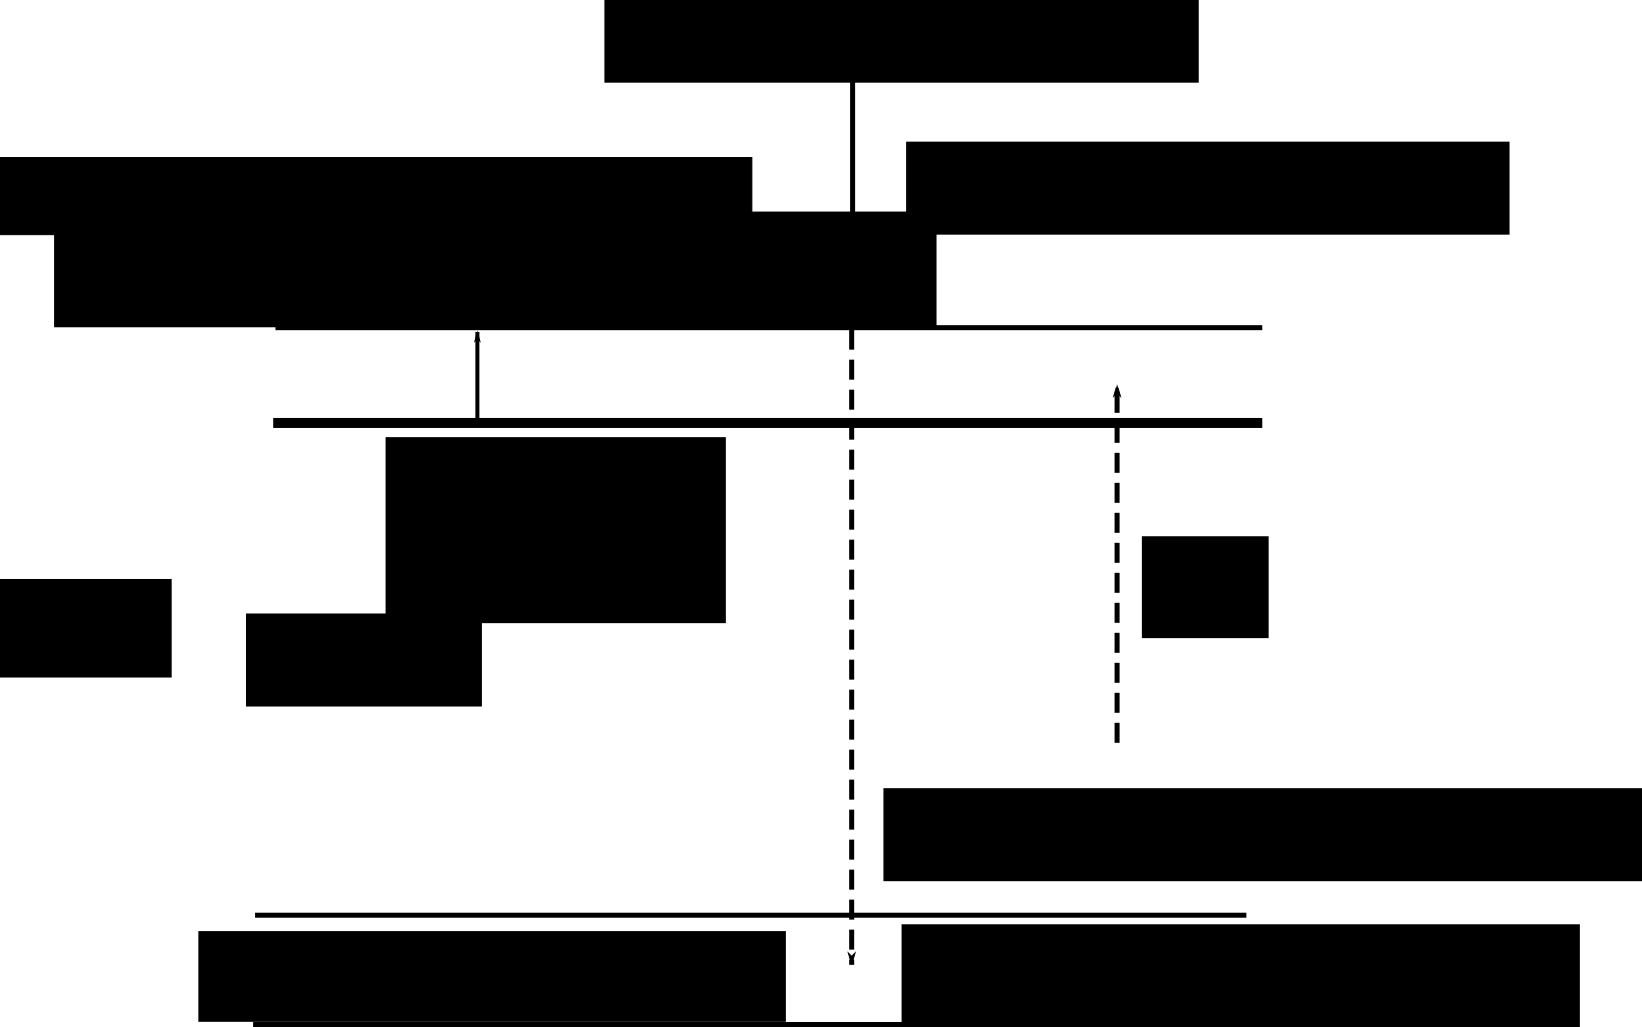
\includegraphics[width=100mm]{grafika/dlcgrowth.pdf}
  \caption{Schématický nákres růstu DLC vrstvy implantací energetických iontů, převzato z \cite{Robertson2002}.}
  \label{dlcgrowth}
\end{figure}

Implantace může navíc probíhat dvěma způsoby, buď přímou implantací dopadajícího atomu, případně srážkou dopadajícího atomu s atomem povrchu a~implantací povrchového atomu do vrstvy (dopadající atom se odrazí). V případě molekulárního iontu (například acetylenu) dojde při srážce s povrchem k~disociaci molekuly a~implantaci každého atomu samostatně, přičemž kinetická energie se mezi ně rozdělí rovnoměrně \cite{Robertson2002}.

\section{Růst DLC vrstev s vodíkem}
Růst DLC vrstev s vodíkem je poněkud složitější než růst čistě uhlíkových vrstev. Podobně jako u čistě uhlíkových vrstev je i zde silná závislost na urychlovacím napětí a~z toho plyne, že klíčovou úlohu opět hrají ionty. U depozic uhlovodíkových vrstev bývá tok iontů $\Phi$ mnohem menší než u čistě uhlíkových vrstev, typicky kolem 10\,\%, zbytek tvoří neutrální molekuly a~atomy \cite{Koidl1991}. 
Pro depozice uhlovodíkových vrstev je typický posuv maxima tvrdosti (tedy i sp$^3$ koncentrace) v~závislosti na energii iontu podle použitého depozičního plynu. Konkrétně to závisí především na jeho molekulové hmotnosti. 
Celková molekulová hmotnost je důležitá proto, že vlastnosti výsledné vrstvy závisí hlavně na energii dopadu v~přepočtu na jeden atom, a~tak například benzenový iont C$_6$H$_6^+$ potřebuje přibližně šestkrát vyšší napětí pro urychlení než iont methanu CH$_3^+$. 
Při nárazu na povrch vrstvy dochází k~disociaci molekuly a~rozdělení energie mezi jednotlivé atomy podle zákona zachování hybnosti. Každý atom se potom implantuje samostatně. Některé další reakce při růstu vrstvy shrnuje obrázek \ref{dlcgrowthH}. Kromě C$_x$H$_y$ iontů jsou mezi dopadajícími částicemi i H atomy a~ionty, C$_x$H$_y$ radikály a~neutrální molekuly.

Povrch rostoucí vrstvy je plně pasivován C--H vazbami, dopadající monoradikály se proto mohou navázat pouze na povrchové volné vazby. Radikály se dvěma volnými vazbami se mohou navázat do existující C--C nebo C--H vazby. Pro neutrální molekuly jako CH$_4$ a~H$_2$ k~žádným reakcím s vrstvou nedochází. Volné vazby na povrchu jsou vytvářeny buď vyražením atomárního vodíku při nárazu iontu a~nebo reakcí s atomárním vodíkem a~vznikem H$_2$ molekuly \cite{Keudell2001}. Díky své velikosti mohou atomy a~atomární ionty vodíku také pronikat do vrstvy a~způsobovat reakce ve vrstvě. Opět může docházet ke vzniku molekulárního vodíku a~volné vazby, případně k~repasivaci již existujících volných vazeb. Dopadající vodíkové atomy také způsobují leptání vrstvy a~zpomalují rychlost růstu \cite{Keudell1996}.

\begin{figure}[btp]
  \centering
  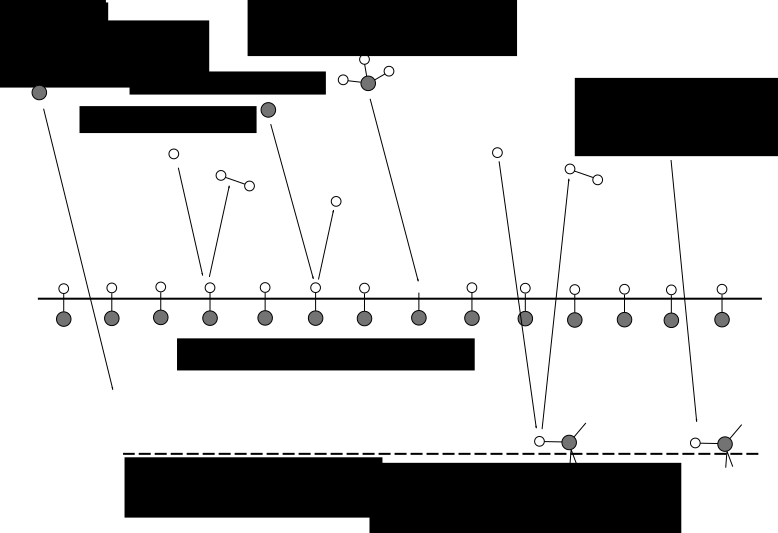
\includegraphics[width=150mm]{grafika/dlcgrowthH.pdf}
  \caption{Schématický nákres procesů růstu DLC vrstev s vodíkem, převzato z \cite{Robertson2002}.}
  \label{dlcgrowthH}
\end{figure}

Mezi klíčové parametry depozice patří vhodná volba depozičního plynu. Běžně používané plyny pro depozice DLC vrstev jsou jednoduché uhlovodíkové sloučeniny jako alkany (např. methan, ethan, propan, butan ...), alkeny (např. ethen), alkyny (např. acetylen), aromatické uhlovodíky (benzen) a~další. Důležité parametry použitého plynu jsou ionizační energie, molekulární hmotnost a~poměr vodíku k~uhlíku. Pro nižší ionizační energie se rychlost depozice zvětšuje přibližně exponenciálně \cite{Koidl1991}. Z poměru uhlíku a~vodíku se pak odvíjí poměr uhlíku a~vodíku ve výsledné vrstvě a~molekulární hmotnost určuje potřebné urychlovací napětí.

Pro depozice tvrdých ochranných vrstev se nejčastěji používá acetylen (C$_2$H$_2$), protože má po methanu nejnižší molekulovou hmotnost, nízkou ionizační energii a~nízký obsah vodíku. Nevýhoda je, že není dostupný v~čisté formě, a~obsahuje některé nečistoty jako například dusík \cite{Conway2000}. Z toho důvodu je pro depozici vrstev určených k~optické charakterizaci nevhodný. Pro depozice vrstev byl proto zvolen methan, který má sice vysokou ionizační energii (cca 12,4\,V), ale neobsahuje příměsi a~kvůli jeho nízké molekulární hmotnosti není potřeba příliš velké urychlovací napětí při depozici.

\section{Kapacitně vázaný vysokofrekvenční doutnavý výboj}
\label{ccp}

Jedná se o jeden z nejvíce používaných typů nízkotlakých výbojů pro depozici DLC vrstev. Je udržován radiofrekvenčním (rf) napětím. Energie z vnějšího obvodu je vázána do výboje přes kapacitní stěnovou vrstvu. V nejjednodušším uspořádání jsou nad sebou umístěny dvě elektrody. Na jednu z nich je přivedeno střídavé napětí, druhá je uzemněná. Vnější obvod také obsahuje blokovací kondenzátor, který zamezuje průchodu stejnosměrného proudu obvodem, a~přizpůsobovací člen, který zajišťuje přizpůsobení impedance zátěže k~výstupní impedanci generátoru. Schéma typického reaktoru je na obrázku \ref{reaktor-schema}. 

\begin{figure}[btp]
  \centering
  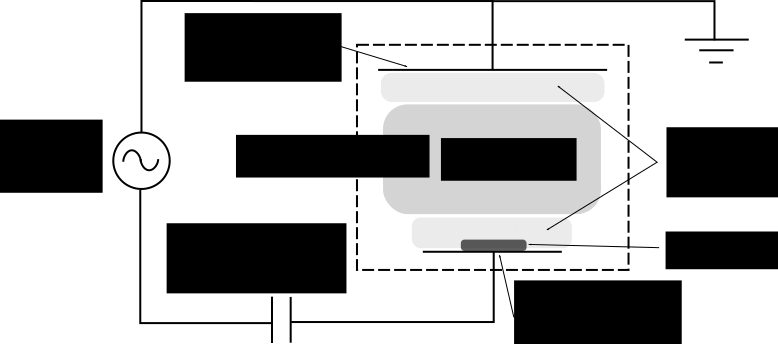
\includegraphics[width=120mm]{grafika/reaktor.pdf}
  \caption{Schéma reaktoru pro vysokofrekvenční kapacitně vázaný výboj.}
  \label{reaktor-schema}
\end{figure}

Rf výboj je pro PECVD výhodný jednak proto, že nedochází k~nabíjení rostoucích dielektrických vrstev (a tedy k úbytku napětí) a~je také poměrně lehké dosáhnout vysokých urychlujících napětí. Typickým projevem rf výboje je totiž vytvoření stejnosměrného samopředpětí $U_b$ na elektrodě, které urychluje ionty směrem k elektrodě. Pro pochopení tohoto jevu je důležité studovat tzv. stěnovou vrstvu, která vzniká u povrchu pevných látek, které jsou v kontaktu s plazmatem. Vznik stěnové vrstvy je typický pro jakékoli plazma a~neomezuje se na vysokofrekvenční výboj. Vznik stěnové vrstvy je způsoben tím, že elektrony mají výrazně vyšší pohyblivost než ionty, proto je tok elektronů na stěny a~elektrody řádově vyšší a~dojde k~jejich nabití záporným nábojem. K~tomu jsou přitahovány kladné ionty z plazmatu a~elektrony jsou naopak odpuzovány, až dojde ke kompenzaci toku elektronů i iontů způsobených rozdílnou pohyblivostí. Mezi plazmou a~povrchem tak vzniká oblast ve které je rozdílná koncentrace iontů a~elektronů a~potenciál v~ní klesá od potenciálu plazmatu na potenciál povrchu. Nejedná se už o plazma, protože to je z definice kvazineutrální.

Další faktor, který hraje roli pro samopředpětí $U_b$ je rozdílná velikost elektrod, protože od ní se odvíjí kapacitance stěnových vrstev a dělení napěťového spádu. Pro $U_b$ platí \cite{Zajickova2006}

\begin{equation}
U_b = 0,83 V_\mathrm{rf} \frac{\xi^q - 1}{\xi^q + 1} \text{,}
\end{equation}
kde $V_\mathrm{rf}$ je amplituda rf napětí, $\xi$ je poměr ploch elektrod a $q$ je konstanta, která závisí na modelu stěnové vrstvy.

Jak již bylo zmíněno výše, pro depozici DLC vrstev s vysokým obsahem sp$^3$ uhlíku je ideální vysoce ionizovaný iontový svazek s úzkým rozdělením energií. V běžném vysokofrekvenčním kapacitně vázaném doutnavém výboji je nicméně obtížné těchto obou parametrů dosáhnout zároveň. Ionty totiž ztrácejí energii především srážkami ve stěnové vrstvě a~pro vysoké tlaky je tedy větší rozpětí energií dopadajících iontů. Při snižování tlaku ale zase dochází k~úbytku srážek v~plazmatu a~snižování stupně ionizace až k~případnému vyhasnutí plazmatu. Pro dosažení kompromisu je potřeba vhodně regulovat depoziční podmínky. Další možností je pak například aplikace externího magnetického pole pro prodloužení dráhy částic v~plazmatu a~větší stupeň ionizace \cite{liebermandischarge, chen2003sheet}.



\cleardoublepage
